\documentclass[german,proseminar,hyperref,utf8]{zihpub}
\usepackage{copyrightbox}

\author{Eric Niklas Wolf}
\title{Score-P Control via Cmake}
\matno{5006150}
\betreuer{William Robert Williams}
\bibfiles{references}
\copyrighterklaerung{\correctme{TODO}}

\begin{document}
    \section{Einleitung}
    \subsection{Ziel und Motivation der Arbeit}
    Profiling und die damit verbundenen Analysewerkzeuge sind essenziell für die Erkennung von
    Optimierungspotenzial und das Messen der Effektivität der Umsetzung.

    Da im HPC Umfeld Ausführungsgeschwindigkeit und Effizienz besonders hohe Prioritäten haben existieren
    mehrere~\longcite{Score-P-Paper}{79} Werkzeuge welche auf die dort verwendeten Technologien
    und Pradigmen angepasst sind.

    Jedoch fokussieren sich die meisten Tools auf bestimmte Anwendungsfälle und Technologien,
    was dazu führt dass sie je nach Anwendungsfall in Kombination eingesetzt werden müssen.

    Dies wiederum kann dazu führen dass eine Anwendung mehrfach mit unterschiedlichen Werzeugen
    analysiert werden muss wenn diese inkompatibel zueinander sind, was wiederum Redundanz
    und Mehraufwand bedeutet.

    Um dies zu vermeiden stellt Score-P~\cite{Score-P-Paper} ein Framework dar welches erlaubt
    eine Anwendung  einmalig zu instrumentisieren und die gewonnenen Daten mit mehreren
    unterschiedlichen Werzeugen zu analysieren.

    Gleichzeitig nutzen viele Projekte Werzeuge welche das Erstellen und Verwalten einen Projektes
    vereinfachen.

    Ein populäres Werkzeug ist CMake~\cite{CMake-Documentation}, für welches jedoch die Nutzung
    von Score-P manuelle Eingriffe und damit zusätzlichen Aufwand benötigt.

    Das Ziel dieses Proseminars ist ein Modul für CMake zu entwickeln welches diesen Aufwand
    reduziert.


    \subsection{Aufbau}
    Dieses Dokument ist wie folgt aufgebaut.

    Zuerst werden die beiden wichtigsten Technologien (Score-P und CMake) betrachtet um einen
    Überblick über deren Funktionsweise zu geben.

    Anschlie{\ss}end werden die im Rahmen dieses Proseminars geschriebenen Module betrachtet
    und mit der bisherigen Verwendung von Score-P verglichen.

    Zum Schluss wird ein Fazit gezogen und ein Ausblick auf weitere Entwicklungen gegeben.

    \newpage
    \section{Betrachtung Score-P}
    \subsection{Architektur}
    Score-P besteht aus mehreren Komponenten, welche in~\ref{fig:score-p-overview} dargestellt
    und anschlie{\ss}end vorgestellt werden.

    \begin{figure}[ht]
        \begin{center}
            \copyrightbox[b]
                {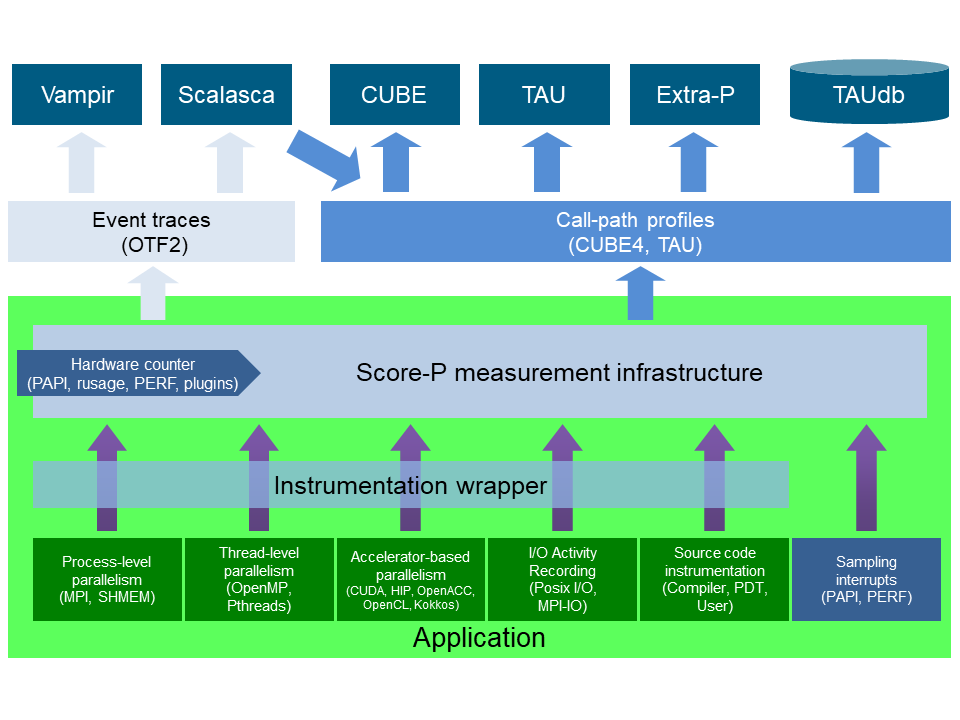
\includegraphics[width=0.75\textwidth]{graphics/score-p-overview.png}}
                {\tiny \url{https://perftools.pages.jsc.fz-juelich.de/cicd/scorep/tags/latest/html/score-p-overview.png}}
            \caption{Score-P Komponenten}
            \label{fig:score-p-overview}
        \end{center}
    \end{figure}

    Der Kern von Score-P besteht aus einer gemeinsamen Messinfrastruktur und darauf aufbauenden
    Integrationen mit unterschiedlichen Profilingschnittstellen.

    Die gesammelten Daten werden wiederum in offenen Datenformaten gespeichert und können
    dadurch von mehreren Werkzeugen verwendet werden.

    \subsubsection{Profilingschnittstellen}
    Neben manueller Instrumentisierung durch den Benutzer~\longcite{Score-P-Documentation}{Application Instrumentation}
    besitzt Score-P Integrationen mit folgenden Technologien.

    \paragraph{Compilerinstrumentisierung}
    Um Aufrufe von Funktionen aufzuzeichnen kann Score-P den verwendeten Compiler
    anweisen das Betreten und Verlassen dieser durch Aufrufe spezieller Funktionen
    zu markieren~\longcite{Score-P-Documentation}{Application Instrumentation}.

    Dabei ist zu beachten das die Namen der entstehenden Regionen und Art wie diese generiert
    werden von dem verwendeten Compiler abhängig ist.

    Dies ist besonders wichtig wenn die zu instrumentisierende Anwendung in C++ geschrieben ist,
    weil einige Compiler kein Filtern der zu instrumentisierenden Funktionen erlauben und C++
    Anwendungen häufig viele kleine Funktionen besitzen wessen Instrumentisierung einen signifikanten
    Overhead erzeugen kann~\longcite{Score-P-Documentation}{Application Instrumentation}.

    \paragraph{MPI Bibliotheksaufrufe}
    Bei MPI handelt es sich um eine standardisierte Schnittstelle für den Nachrichtenaustausch
    zwischen parallel ablaufenden Prozessen mit eigenen Adressbereichen~\longcite{mpi}{1}.

    Um Aufrufe von MPI Funktionen zu Erkennen und zu Messen wird dafür das im MPI Standard
    spezifizierte `Profiling Interface'~\shortcite{mpi}{717} verwendet.

    Bei der Instrumentisierung einer Anwendung wird dafür neben der MPI Implementierung zusätzlich
    gegen eine von Score-P bereitgestellte Bibliothek gelinkt~\longcite{Score-P-Documentation}{Application Instrumentation}.

    \paragraph{SHMEM Bibliotheksaufrufe}
    Bei SHMEM handelt es sich ebenfalls um eine standardisierte Schnittstelle, bei welcher jedoch
    im Gegensatz zu MPI im Rahmen des `Partitioned Global Address Space' Paradigmas von einem
    einzigen globalen Adressbereich ausgegangen wird welcher auf mehrere Ausführungseinheiten
    verteilt sein kann und Datentransfers einseitig ablaufen~\longcite{openshmem}{1}.

    Um Aufrufe von SHMEM Funktionen zu Erkennen und zu Messen wird wie bei MPI auf ein standardisiertes
    `Profiling Interface'~\shortcite{openshmem}{140} zugegriffen welches ein Linken gegen eine von
    Score-P bereitgestellte Bibliothek erfordert~\longcite{Score-P-Documentation}{Application Instrumentation}.

    \paragraph{OpenMP Direktiven und API Aufrufe}
    OpenMP ist im Gegensatz zu den beiden vorherigen Technologien keine Bibliotheksschnittstelle
    sondern eine API welche neben Funktionen auch aus Compilerdirektiven besteht.

    Damit können Anwendungsentwickler Bereiche des Quellcode explizit zur parallelen Ausführung
    innerhalb eines gemeinsamen Adressbereichs~\longcite{openmp}{23} markieren und die Umsetzung 
    dem verwendeten Compiler überlassen.

    Die Verwendung von Compilerdirektiven stellt jedoch auch eine Hürde bei der Instrumentisierung dar
    weil das Erkennen und Messen von Funktionsaufrufen nicht ausreicht um die komplette API abzudecken.

    Eine der von Score-P verwendeten Lösungen stellt die Opari2 Komponente dar, welche den Quellcode der
    zu instrumentisierenden Anwendung analysiert und Aufrufe von Messfunktionen an bestimmten Stellen
    einfügt~\longcite{Score-P-Documentation}{Introduction}.

    Eine Alternative ist die Verwendung des `OMPT Interface'~\shortcite{openmp}{419}, welches eine
    standardisierte Schnittstelle für die Interaktion mit einer OpenMP Implementierung darstellt.

    Zwar kann dabei auf das Modifizieren von Quellcode und die dadurch entstehende Probleme verzichtet werden,
    jedoch existiert die Schnittstelle erst seit OpenMP 5.0 und wird momentan (Stand 2024) noch nicht von
    GCC, einer weit verbreiteten Compilersammlung, unterstützt~\cite{gomp}. 

    \paragraph{Pthread Bibliotheksaufrufe}
    Pthread, auch bekannt als POSIX Threads, ist die standardisierte Threadingbibliothek auf POSIX
    kompatiblen Betriebssystemen, welche von Score-P durch das Wrappen von Bibliothekssymbolen
    beim Linken der zu instrumentisieren Anwendung mit von Score-P bereitgestellten
    Implementierungen Instrumentisiert wird~\longcite{Score-P-Documentation}{Application Instrumentation}.

    \paragraph{OpenCL Bibliotheksaufrufe}
    Bei OpenCL handelt es sich wie bei MPI und SCHMEM um eine standardisierte Bibliotheksschnittstelle,
    welche es Anwendungsentwicklern erlaubt Berechnungen auf verschiedene Hardware wie u.a. einer GPU
    zu verteilen~\longcite{opencl}{2}.
    
    Dabei wird grundsätzlich von mehreren Adressbereichen ausgegangen~\longcite{openmp}{30}.

    Das Instrumentieren wird wie bei Pthread durch das Wrappen von Bibliothekssymbolen beim
    Linken ermöglicht.

    \paragraph{OpenACC Direktiven und API Aufrufe}
    Die API von OpenACC ähnelt der von OpenMP, weil der Anwendungsentwickler ebenfalls durch
    Compilerdirektiven explizit Teile der Anwendung parallel ablaufen lassen kann.

    Im Gegensatz zu OpenMP konzentriert sich OpenACC jedoch auf heterogene Hardware und besitzt
    dementsprechend meistens keinen gemeinsamen Adressbereich, da die ausgeführten Programmteile
    möglicherweise auf anderen Geräten laufen~\longcite{openacc}{11}.

    Beim Instrumentisieren von Anwendungen welche OpenACC unterstützen verwendet Score-P das
    `Profiling and Error Callback Interface'~\shortcite{openacc}{123}, wofür wiederum gegen eine
    von Score-P bereitgestellte Bibliothek gelinkt~\longcite{Score-P-Documentation}{Introduction}
    werden muss.

    \paragraph{CUDA}
    CUDA ist eine vom Hersteller NVIDIA entwickelte Werzeugsammlung welche es erlaubt GPU-basierte
    Anwendungen zu entwickeln und auszuführen~\longcite{nvidia-docs}{CUDA}.

    Score-P erlaubt das Aufzeichnen von Funktionsaufrufen der CUDA API und GPU Aktivitäten mit Hilfe des
    `CUDA Profiling Tools Interface'~\shortcite{nvidia-docs}{CUPTI}~\longcite{Score-P-Documentation}{Application Measurement}.

    \paragraph{HIP}
    Bei HIP handelt es sich wie bei CUDA um eine Werkzeugsammlung für die Entwicklung von GPU-basierten
    Anwendungen welche vom Hersteller AMD als Bestandteil der ROCm Plattform mit einem Fokus auf
    Kompatibilität mit GPUs von sich selbst und NVIDIA entwickelt wurde~\longcite{rocm-docs}{HIP documentation}.

    Wie bei CUDA unterstützt Score-P das Aufzeichnen von Funktionsaufrufen der ROCm API und GPU Aktivitäten,
    wobei eine nicht näher spezifizierte Schnittstelle verwendet wird~\longcite{Score-P-Documentation}{Application Measurement}.

    \paragraph{I/O}
    Funktionsaufrufe von Funktionen bekannter I/O Schnittstellen können durch Score-P aufgezeichnet werden.

    Dabei werden neben den bekannten POSIX Funktionen auch Funktionen der asynchronen POSIX Schnittstelle,
    ISO C und MPI untersützt~\longcite{Score-P-Documentation}{Introduction}.

    \subsubsection{Datenformate}
    Nach dem Instrumentieren einer Anwendung ermöglicht Score-P zwei Arten der Datenerfassung,
    genannt `tracing' und `profiling'.

    Bei `tracing' werden aufzuzeichnende Ereignisse unter Beibehaltung zeitlicher und örtlicher
    Zusammenhänge im Open Trace Format 2 abgespeichert, welches u.a. von den Werkzeugen Scalasca
    und Vampir verwendet wird~\longcite{Score-P-Documentation}{Application Measurement}.

    Da dies jedoch gro{\ss}e Datenmengen erzeugen kann erlaubt `profiling' das Zusammenfassen von
    Ereignissen innerhalb bestimmter Regionen, wobei die entstehenden Daten im CUBE4 Format
    gespeichert und von Werkzeugen wie Cube und TAU verwendet werden
    können~\longcite{Score-P-Documentation}{Application Measurement}.

    Dabei stellt jede aufgerufene Funktion eine Region dar welche zusammen mit den von ihr
    aufgerufenen Funktionen einen Baum bildet.

    Die entstehenden Aufrufbäume können basierend auf bestimmten Funktionsparametern,
    benutzerdefinierten Phasen und einzelnen Aufrufen weiter unterteilt
    werden~\longcite{Score-P-Documentation}{Application Measurement}.

    \subsection{Anwendung}
    Um eine Anwendung mit Score-P zu instrumentisieren wird ein Befehl namens `scorep' zur Verfügung
    gestellt welcher vor die Befehle zum Compilieren und Linken der Anwendung gestellt wird.

    Das damit assoziierte Programm analysiert den übergebenen Befehl und führt die zur Instrumentisierung
    notwendigen Aktionen aus, wobei die Berechnung von benötigten Linkerargumenten und zu linkenden
    Bibliotheken von einem weiteren Werkzeug namens `scorep-config' durchgeführt wird~\longcite{Score-P-Documentation}
    {Score-P Tools}.

    Die zu nutzenden Profilingschnittstellen werden über Befehlsargumente ausgewählt oder durch
    Analyse des übergebenen Befehls erkannt, wobei dies nicht immer funktioniert~\longcite{Score-P-Documentation}
    {Application Instrumentation}.

    Dabei ist zu beachten dass für jede Instrumentisierte Anwendung nur ein Threadingparadigma
    (OpenMP oder Pthread) und eine Kommunikationsparadigma (MPI oder SHMEM) ausgewählt werden kann
    und es Einschränkungen bei der Verwendung von Profilingschnittstellen in statischen
    Bibliotheken gibt wenn diese nicht beim Erstellen der fertigen Anwendung aktiviert werden.

    Zusätzlich kann die Unterstützung für bestimmte Profilingschnittstellen bei einer Score-P
    Installation fehlen, was durch die Ausgaben des Befehls `scorep-info' überprüft werden kann.

    Au{\ss}erdem kann bei der Verwendung von Werkzeugen wie CMake und Autotools der konfigurierte Compiler
    bereits vor dem Bauen eines Projektes aufgerufen werden um die Verfügbarkeit von Schnittstellen
    oder andere Informationen für das Konfigurieren des Projektes zu erhalten.

    Da bei der Verwendung von Score-P der `scorep' Befehl als Compiler verwendet wird kann es dabei
    zu Fehlern kommen obwohl Score-P in dieser Phase nicht benötigt wird~\longcite{Score-P-Documentation}
    {Score-P Compiler Wrapper Usage}.

    Um dies zu verhindern stellt Score-P Befehle bereit welche sich normalerweise wie der Befehl
    `scorep' verhalten, durch das Setzen von bestimmten Umgebungsvariablen jedoch den Aufruf an den
    verwendeten Compiler durchreichen~\longcite{Score-P-Documentation}{Score-P Compiler Wrapper Usage}.

    \newpage
    \section{Betrachtung CMake}
    \correctme{TODO}


    \newpage
    \section{Implementierung}
    \correctme{TODO}


    \section{Leistungsanalyse}
    \correctme{TODO}


    \section{Fazit}
    \correctme{TODO}


    \section{Ausblick}
    \correctme{TODO}

    \newpage
    \listoffigures
\end{document}
